\documentclass{article} % use option titlepage to get the title on a page of its own.
\usepackage{polski}
\usepackage[utf8]{inputenc}
\usepackage{graphicx}
\usepackage[a4paper, total={7in, 10in}]{geometry}
\usepackage{listings}
\usepackage{amsmath}
\graphicspath{ {./images/} }
\title{Rozwiązywanie Sapera za pomocą sztucznej inteligencji}
\date{04.05.2019}
\author{Dominika Zembrzuska, Kacper Ziółkowski, Mateusz Buchajewicz}
\begin{document}
\maketitle

\section{Wprowadzenie}
Celem projektu jest utworzenie algorytmów opartych na sztucznej inteligencji rozwiązujących popularną grę Saper.
\section{Zasady sapera}
\section{Wykorzystane technologie}
\section{Opis algorytmu}
\subsection{Bot generujący dane}

Bot działa w oparciu o 3 główne metody rozwiązujące:
\begin{itemize}
    \item{Rozwiązywanie za pomocą prostej logiki}
    \item{Rozwiązywanie za pomocą układów równań}
    \item{Strzelanie w losowe pole}    
\end{itemize}
\subsubsection{Rozwiązywanie za pomocą prostej logiki}
Sprawdza po kolei wszystkie pola planszy, zawierające wartość numeryczną. 
Jeśli liczba pól sąsiadujących ze sprawdzanym polem, a nieoznaczonych jako
"bez miny" (czyli zarówno oznaczonych jako "miny", jak i pustych) jest taka
jak wartość pola, to wszystkie te pola są oznaczane jako miny.
Natomiast jeżeli liczba oznaczonych min na polach sąsiadujących jest równa wartości 
sprawdzanego pola, to wszystkie pozostałe pola sąsiadujące zostają oznaczone jako "bez miny"
\newpage
\subsubsection{Rozwiązywanie za pomocą układów równań}
Metoda opiera się na ułożeniu układu równań z pól na planszy oraz rozwiązaniu go. 
Algorytm przekształca układ równań na macierz n x m, gdzie n jest liczbą oznaczonych 
pól z wyznaczoną wartością, a m jest liczbą różnych pól nieoznaczonych z nimi sąsiadujących.\\
Dla przykładu, poniższa plansza:
\begin{figure}[h]
    \centering
    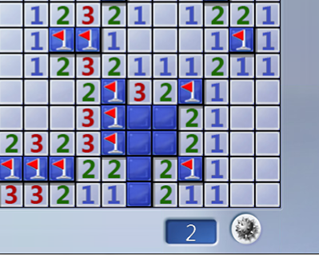
\includegraphics[scale=0.5]{matrix_first.png}
    \caption{Przykładowa plansza sapera}
\end{figure} \\
Zostanie przekształcona do postaci:\\
\begin{figure}[h]
    \centering
    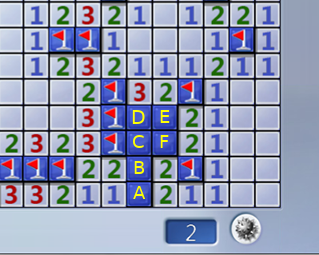
\includegraphics[scale=0.5]{matrix_marked.png}
    \caption{Przykładowa plansza sapera z polami oznaczonymi jako zmienne}
\end{figure} \\
Otrzymany układ równań: \\
$$
\begin{cases}
 A + B = 1 \\
 A + B + C = 1 \\
 D + E = 1 \\
 E + F = 1 \\
 A + B + C + F = 1 \\
\end{cases}
$$

Co z kolei można zapisać w postaci macierzy: \\

\[
\begin{bmatrix}
    1 & 1 & 0 & 0 & 0 & 0 \\
    1 & 1 & 1 & 0 & 0 & 0 \\
    0 & 0 & 0 & 1 & 1 & 0 \\
    0 & 0 & 0 & 0 & 1 & 1 \\
    1 & 1 & 1 & 0 & 0 & 1 \\
\end{bmatrix}
\begin{bmatrix}
    A \\ B \\ C \\ D \\ E \\ F\\
\end{bmatrix}
=
\begin{bmatrix}
    1 \\ 1 \\ 1 \\ 1 \\ 1 \\
\end{bmatrix}
\]

Macierz główna nie jest macierzą kwadratową (a przynajmniej nie zawsze), 
więc algorytm nie może określić dokładnych wartości wszystkich zmiennych. Może jednak 
przekształcić tę macierz za pomocą operacji elementarnych do takiej postaci, żeby
mógł odczytać z niej jak najwięcej wartości zmiennych. 
\[
\begin{bmatrix}
    1 & 1 & 0 & 0 & 0 & 0 & | & 1\\
    1 & 1 & 1 & 0 & 0 & 0 & | & 1\\
    0 & 0 & 0 & 1 & 1 & 0 & | & 1 \\
    0 & 0 & 0 & 0 & 1 & 1 & | & 1\\
    1 & 1 & 1 & 0 & 0 & 1 & | & 1\\
\end{bmatrix}
\longrightarrow
\begin{bmatrix}
    1 & 1 & 0 & 0 & 0 & 0 & | & 1\\
    0 & 0 & 1 & 0 & 0 & 0 & | & 0\\
    0 & 0 & 0 & 1 & 0 & 0 & | & 0 \\
    0 & 0 & 0 & 0 & 1 & 0 & | & 1\\
    0 & 0 & 0 & 0 & 0 & 1 & | & 0\\
\end{bmatrix}
\] \\
Co jest tożsame z układem równań:\\
$$
\begin{cases}
 A + B = 1 \\
 C = 0 \\
 D = 0 \\
 E = 1 \\
 F = 0 \\
\end{cases}
$$

W tym przypadku doskonale widać, że pole E zawiera minę, natomiast pola C, D, F jej nie zawierają. 
O polach A i B nic nie wiadomo, co wynika z faktu iż macierz główna nie jest kwadratowa. \\
Warto jednak zauważyć, że operacje podstawowe nie zawsze zwrócą wartość 0 lub 1. W ogólności
algorytm sprawdza otrzymane wyniki za pomocą prostych warunków: 
$$
\begin{cases}
 \text{if } \forall{(a_{i} \in M_{j}^W)} \text{ } |\sum{a_{i}}| = \sum{|a_{i}| = |b_{j}|}  \text{ then } x_{j}=1 \\
 \text{if } \forall{(a_{i} \in M_{j}^W)} \text{ } |\sum{a_{i}}| = \sum{|a_{i}|} = 0 \text{ then } x_{j}=0 \\
\end{cases}
$$

Analogicznie jak wyżej, wszystkie pola z wartością 1 algorytm oznacza jako pola "z miną", a te z wartością 0 jako "bez miny".

\subsubsection{Strzelanie w losowe pole}
Ta metoda jest używana wtedy i tylko wtedy, gdy obie powyższe po przejrzeniu całej planszy
nie dadzą rady oznaczyć ani jednego pola. Algorytm wybiera losowo jedno z nieoznaczonych pól
i oznacza je jako pole "bez miny". Jeśli oznaczy poprawnie gra jest kontynuowana z wykorzystaniem
 powyższych metod. Jeśli pole nie zostało poprawnie oznaczone, gra jest zakończona porażką.

\subsection{Sieć neuronowa}
\subsection{Prolog}
\section{Porównanie metod}
Bot osiąga około 85-90\% skuteczności na małych planszach (10x10, 10 min) 
oraz około 10-15\% na dużych planszach (30x15, 99 min).
\begin{center} 
    \begin{tabular}  { | l | c | r |   }
        \hline
        Algorytm & Mała & Duża  \\
        \hline
        Bot & 85-90 & 10-15 \\
        \hline
        Sieć neuronowa & ? & ? \\
        \hline
        Logika / prolog & ? & ? \\
        \hline
    \end{tabular}
\end{center}
\section{Wnioski}
\end{document}